\PassOptionsToPackage{utf8}{inputenc}
\documentclass{bioinfo}

\usepackage{natbib}
%\usepackage[
%backend=biber,
%sorting=ynt
%]{biblatex}

\usepackage{makecell}

\usepackage{floatrow}

\usepackage{comment}

\usepackage{siunitx}

% singlelinecheck=false puts subcaptions on the left
\usepackage[singlelinecheck=false]{subcaption}

\usepackage[usenames,dvipsnames]{xcolor}

%\usepackage{amsthm}
% Says package is already imported?
\theoremstyle{definition}
\newtheorem{definition}{Definition}[section]
\newtheorem{theorem}{Theorem}[section]
\newtheorem{corollary}{Corollary}[theorem]
\newtheorem{lemma}[theorem]{Lemma}

\usepackage{algorithm2e}
\SetKwRepeat{Do}{do}{while}%

% we squeeze our figures even more together
\captionsetup{belowskip=-2pt}

\SetAlgoLined
\SetKwProg{MyStruct}{Struct}{ contains}{end}

\newcommand{\vocab}{\textbf}
\newcommand{\red}[1]{{\textcolor{Red}{#1}}}
\newcommand{\FIXME}[1]{\red{[FIXME: #1]}}

\usepackage{orcidlink}
\hypersetup{hidelinks}


\usepackage{graphicx}

\def\labelitemi{--}

\copyrightyear{2023} \pubyear{XXXX}

\access{Advance Access Publication Date: Day Month Year}
\appnotes{Genome Analysis}

\begin{document}
\firstpage{1}

\subtitle{Genome Analysis}

\title[FantasticLamp]{FantasticLamp: a genome graph based pipeline for calculating the efficacy of genomic edits}
\author[Schutte \textit{et~al}.]{

Casper~Schutte\,$^{\orcidlink{0000-0003-4245-6842}\text{\sfb 1}}$,
Erik~Garrison\,$^{\orcidlink{0000-0003-3821-631X}\text{\sfb 2}*}$,
Ian~T~Fiddes\,$^{\orcidlink{0000-0002-1580-7443}\text{\sfb 3}}$

}

\address{
$^{\text{\sf 1}}$Department of Bioinformatics and Computational Biology, University of Stellenbosch, Stellenbosch, 7600, Western Cape, South Africa \\
$^{\text{\sf 2}}$Department of Genetics, Genomics and Informatics, University of Tennessee Health Science Center, Memphis, 38163, Tennessee, USA \\
$^{\text{\sf 3}}$Ian's affiliation goes here \\
%
}

\corresp{
$^\ast$To whom correspondence should be addressed. \\
% $^\dagger$Contributed equally.\
}

\history{Received on XXXXX; revised on XXXXX; accepted on XXXXX}

\editor{Associate Editor: XXXXXXX}

\abstract{
\textbf{Motivation:}
Accurately calculating the efficacy of genomic edits is crucial to understanding the performance of the editing techniques, in order to optimize methods and improve the success rate of the edits.
Additionally, by understanding the success rate of genomic edits, researchers can identify any potential problems or limitations of the techniques and work to overcome them.
This can help to improve the accuracy and precision of the editing methods, which is essential for many applications, such as creating genetically engineered cells for therapeutic purposes, understanding gene functions, and studying genetic diversity in a population of cells. Current linear alignment methods for quantifying the success of edits suffer from reference bias and fail to capture the complexity involved when dealing with multiple edit states.\\
% Mention current methods and why there is need for better methods.
\textbf{Results:}
We design \textit{FantasticLamp}, an open source genome-graph-based pipeline for calculating the efficacy of genomic edits performed on multiple populations of cells.
It constructs a variation graph from the reference genome and edit template sequences that includes both edited and unedited sequences as paths, and combinations of edits as potential walks through the graph.
It then maps reads from the edited populations onto this graph in order to calculate the coverage of the edited sequences compared to the unedited sequences.
This pipeline aims to provide a quantitative measure of the success of each genomic edit without bias towards the reference or particular single editing constructs.\\
% Reword this paragraph, add detail regarding the process. Mention the successful implementation.
\textbf{Availability:}
\textit{FantasticLamp} is published as free software under the MIT open source license.
Source code and documentation are available at \url{https://github.com/casper-schutte/fantastic-lamp}.
\textbf{Contact:} \href{egarris5@uthsc.edu}{egarris5@uthsc.edu} \\
%\textbf{Supplementary information:} Supplementary data are available at \textit{Bioinformatics} online.
}

\maketitle


\section{Introduction}
\label{sec:introduction}
In the field of genome engineering, researchers often perform genomic edits in cells, such as CRISPR/Cas9, TALEN, and ZNF-based systems, to study gene functions and to create new cell lines \citep{gaj2013zfn}.
However, these edits may not always be successful, and it may be challenging to identify and quantify the success rate of these edits in large-scale data sets \citep{guell2014genome}, \citep{van2020delivery}.
Linear approaches that attempt to consider all possible edit states as individual sequences in order to accurately represent complexity can become overly complex themselves and prone to errors \citep{huang2013short}, \citep{mun2021leviosam}.
Additionally, when assessing the success rate of genomic edits, a linear alignment method may introduce reference bias and overlook the complexity of edits, particularly when multiple nearby edits and edit state mixtures are present.


Alternatively, a genome graph approach can provide a more complete and accurate perspective of sequence relationships, while avoiding reference bias and capturing all allele state mixtures present within the targeted edits, even in the case of overlapped edits \citep{eggertsson2017graphtyper}.

Compared to linear alignment methods, genome graphs can provide a more accurate and comprehensive view \citep{garrison2018variation} of the relationships between sequences \citep{paten2017genome} because reads can be mapped to a graph that captures the variation between all the genomes/subsequences, instead of to a single reference, as seen in Figure \ref{fig:images} (A), (B), and (C).
The cost of this increased accuracy and the ability to represent complexity is that using genome graphs is more computationally intensive than linear alignments methods \citep{rakocevic2019fast}.

Given these advantages over linear methods, we suggest a pipeline based on genome graph alignment tools would be more effective/better suited for quantifying edit efficacy in multiple populations of edited cells. 

% To add:
% Have I covered:
% Enough backround info (what are we doing?)
% Expanding on motivation (why are we doing this?) More detail on why graphs are better?
% Briefly, how we did/will do this? 


Here, we present \textit{FantasticLamp}, a simple pipeline that uses genome graph based sequence analysis to calculate/quantify edit efficacy in experiments where multiple edits were performed separately on the same population (wording?). 
% wording? Detail?



\section{Implementation}
\label{sec:implementation}
Here we describe the steps and tools used in creating \textit{FantasticLamp}. 



Given a reference genome and reads sequenced from multiple edited populations, the pipeline uses a design library CSV file, which contains the intended edits and reference sequences at the intended edit sites, to construct a genome graph.

The genome graph is made up of the reference genome, the intended edit sequences (`homology arms', or `edit homology arms'), and the reference sequences at the edit sites (`reference homology arms').
The construction of the graph involves taking the homology arms and reference homology arms and mapping them to the reference genome using \textit{minimap2} \citep{li2018minimap2}.
%Minimap: 
The inclusion of the reference homology arms is what allows the pipeline to calculate the relative coverage (and thus the edit efficiency) by comparing the edit homology arm coverage to the reference homology arm coverage.

A variation graph is then induced by \textit{seqwish} \citep{garrison2023unbiased} that represents the relationships between the reference genome and both groups of homology arms (reference and edit).
Before the graph is constructed, the nodes are 'chopped' into segments smaller than 256 base pairs and then the graph is sorted using \textit{odgi} \citep{guarracino2022odgi}.
These steps are necessary in order for the graph to then be constructed, again using \textit{odgi}. 

The graph is converted into a format that is more efficient and finally indexed, both steps using \textit{vg} \citep{garrison2018variation}.
The pipeline then maps reads from the edited populations to this graph using \textit{vg}, creating a GAF (Gene Annotation Format) file representing the alignment.
A Python script is called to parse the alignment file and calculate the coverage of the homology arms compared to the reference homology arms.
The output of this pipeline is a coverage table in the form of a TSV file, which displays the name of each intended edit sequence along with the homology arm coverage and reference homology arm coverage providing a quantitative measure of the efficacy of each edit.
  

This allows \textit{FantasticLamp} to simultaneously quantify the efficacy of edits in multiple edited populations, which can be used to test novel editing methods as well as to verify current methods in experiments that involve genomic edits.
By using reads aligned to a graph instead of linear alignment, \textit{FantasticLamp} can avoid reference bias, making it a useful tool for researchers in the field of genome engineering and other related fields who wish to precisely quantify genome edit states.\\
A flow diagram of the steps and files used in the \textit{FantasticLamp} pipeline can be seen in Figure \ref{fig:images}(D).


%We will discuss the tools used, not in extreme detail but enough to justify and explain their use.
% Mention important functions or at least describe how coverage is calculted, etc. Mention problem of shared reads, plasmid integration, etc.

\section{Results}
\label{sec:results}
%This pipeline was initially tested and developed using a data set containing sequencing reads %(mention platform) from experiments where multiple edits (insertions, deletions, and substitutions) were performed on a population of \textit{Saccharomyces cerevisiae} (check this) by Inscripta Inc. (ref?). 
%The initial/preliminary results showed/demonstrated/indicated the pipeline's ability to calculate read coverage (and thus efficacy) of the edits performed. 
%Unfortunately, logistical issues prevented continued use of this data set and an artificial test data set was constructed. This artificial data set was comprised of a tiny reference genome, an accompanying design library CSV file containing reference sequences from the genome and edited sequences, and artificial reads mapping to either the reference or the edit at a particular edit locus. 
%The pipeline accurately calculated the edit coverage and thus provided a quantitative measure of edit efficacy.  

The initial development and testing of this pipeline were carried out using a dataset containing sequencing reads from various experiments. These experiments involved multiple alterations - insertions, deletions, and substitutions - on a population of \textit{Saccharomyces cerevisiae}. They were performed in distinct batches by Inscripta Inc. (reference pending).

Preliminary results demonstrated the pipeline's capacity to calculate the read coverage, which acted as a measure of the effectiveness of the implemented edits.
However, due to unforeseen logistical constraints, further usage of this dataset was halted. Consequently, an artificial dataset was constructed for further testing and refinement.

This synthetic dataset encompassed a small reference genome, a related design library CSV, which contained both the reference and edited sequences from the genome, and artificial reads mapping to either the reference or the edit at a specific edit locus. 
Notably, the pipeline was successful in accurately calculating the edit coverage from this dataset, providing a quantitative evaluation of the edit's effectiveness.

%\begin{figure}
%	\centering
%	\fbox{\includegraphics[width=\columnwidth]{flow.pdf}}
%	\caption{Test Caption for Insertion}
%	\label{fig:insert}
%\end{figure}

%\begin{figure}
%	\fbox{\includegraphics{deletion.pdf}}
%	\caption{Test Caption for Deletion}
%	\label{fig:deletion}
%\end{figure}
%
%\begin{figure}
%	\fbox{\includegraphics{substitution.pdf}}
%	\caption{Test Caption for Substitution}
%	\label{fig:substitution}
%\end{figure}


\begin{figure}[htbp]
	\centering
	\begin{minipage}[b]{0.35\columnwidth}
		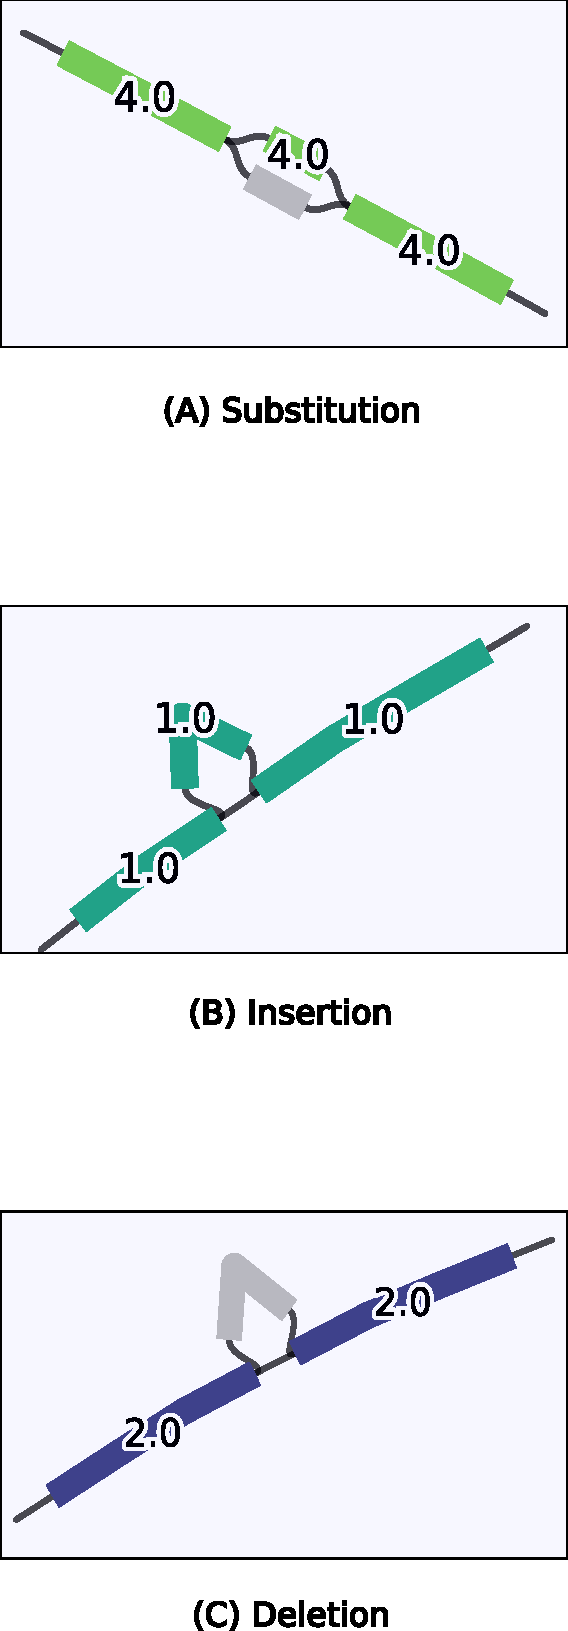
\includegraphics[width=\textwidth]{panels.pdf}
		%\caption{Test caption for panel figure}
		\label{fig:panel}
	\end{minipage}
	\hfill
	\begin{minipage}[b]{0.64\columnwidth}
		\centering
		\fbox{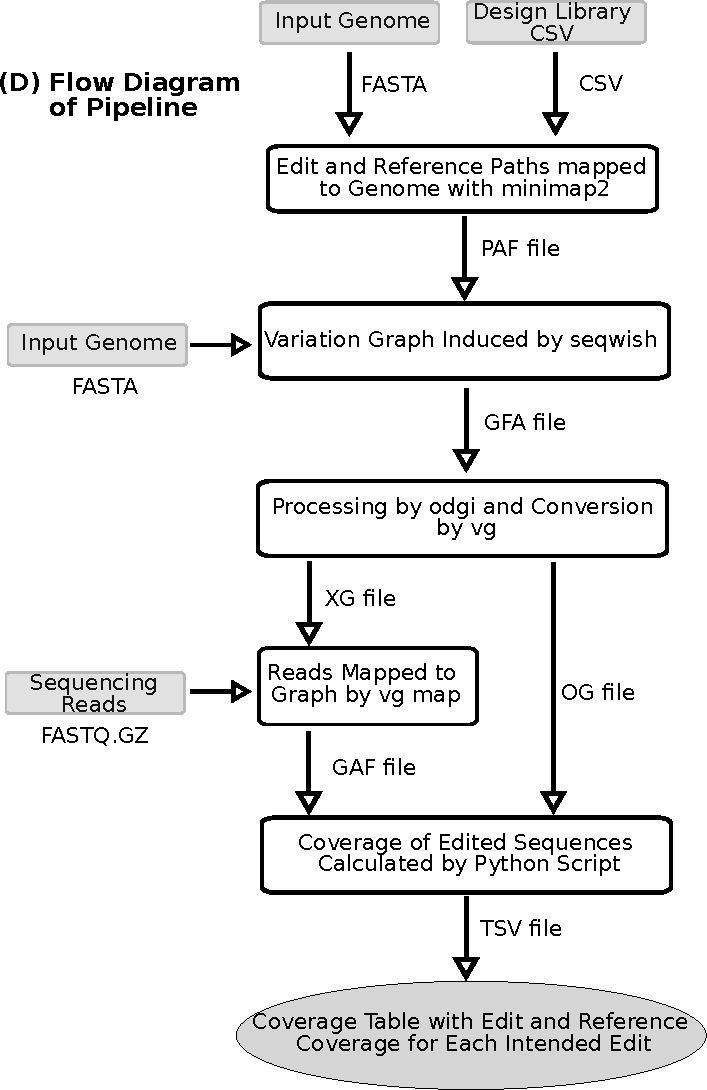
\includegraphics[width=\textwidth]{flow_test.pdf}}
		%\caption{Test caption for flow diagram}
		\label{fig:flow}
	\end{minipage}
	\caption{(A) Graph representation of a substitution. Edit path shown in green. (B) Graph representation of an insertion. Edit path shown in light blue. (C) Graph representation of a deletion. Edit path shown in dark blue. (D) Diagram depicting the steps, software tools, and file formats use in the \textit{FantasticLamp} pipeline.}
	\label{fig:images}
\end{figure}



\section{Discussion}
\label{sec:discussion}
As novel genome editing processes are developed in the near future, we posit that the need for software tools that can capture the complexity of the edits and the relationship between them will increase.
We show a basic approach for quantifying complex genome editing results, which are difficult to reliably and simply evaluate using a single reference genome that may lead to biased estimates of edit states.
The design library CSV file used in the creation of this pipeline was unique to a specific set of editing experiments performed at Inscripta Inc.
However, the basic format is generic to other editing experiments that users may carry out in the future, with only minimal changes to the script to adjust for difference in formatting of the design library file.
Future users will have to edit the bash script `find\_coverage.sh' such that the correct columns containing the edit- and reference homology arms are extracted.
While the pipeline was tested on artificial data and singleplex sequencing data, it is possible to perform analysis using pooled sequencing data, but data availability has limited our ability to thoroughly test this.
In summary, \textit{FantasticLamp} provides a basic demonstration of the principle of using a variation graph as a reference system to avoid bias when quantifying genomic edits, and stands as a prototype for future work in this space.
\section*{Acknowledgements}
We are grateful to Inscripta Inc for providing the data from editing experiments that was used to create and test this pipeline. We thank Deanna Church for supporting our collaboration.

\section*{Funding}

% Don't think this applies? Check with Erik
\section*{Data availability}
Code and links to data resources used to build this manuscript and its figures can be found in the paper's public repository: \url{https://github.com/casper-schutte/fantastic-lamp}.


\bibliographystyle{natbib}
\bibliography{document}

\end{document}
